\documentclass[a4paper]{article} 
\addtolength{\hoffset}{-2.25cm}
\addtolength{\textwidth}{4.5cm}
\addtolength{\voffset}{-3.25cm}
\addtolength{\textheight}{5cm}
\setlength{\parskip}{0pt}
\setlength{\parindent}{0in}

\usepackage{natbib}
\usepackage{blindtext} % Package to generate dummy text
\usepackage{charter} % Use the Charter font
% \usepackage[utf8]{inputenc} % Use UTF-8 encoding
\usepackage{microtype} % Slightly tweak font spacing for aesthetics
\usepackage{amsthm, amsmath, amssymb} % Mathematical typesetting
\usepackage{float} % Improved interface for floating objects
\usepackage{hyperref} % For hyperlinks in the PDF
\usepackage{graphicx, multicol, multirow} % Enhanced support for graphics
%\usepackage{xcolor} % Driver-independent color extensions
\usepackage{pseudocode} % Environment for specifying algorithms in a natural way
\usepackage[ddmmyyyy]{datetime} % Uses YEAR-MONTH-DAY format for dates
%\usepackage{gensymb}
\usepackage{bibentry}
\usepackage{color}
\usepackage{booktabs}
\usepackage{enumitem}
\usepackage{tikz}
\usepackage{psfrag}
\usepackage{forest}
\usepackage{makecell}
\usepackage{adjustbox}
\usepackage{xeCJK}
% \setCJKmainfont{Noto Serif CJK SC}
% \setCJKmonofont{Noto Sans Mono CJK SC}
\setCJKmainfont{SimSun}
\setCJKmonofont{SimSun-ExtB}

\usepackage{fancyhdr} % Headers and footers
\pagestyle{fancy} % All pages have headers and footers
\fancyhead{}\renewcommand{\headrulewidth}{0pt} % Blank out the default header
\fancyfoot[L]{} % Custom footer text
\fancyfoot[C]{} % Custom footer text
\fancyfoot[R]{\thepage} % Custom footer text
\newcommand{\note}[1]{\marginpar{\scriptsize \textcolor{red}{#1}}} % Enables comments in red on margin

\renewenvironment{abstract}{\vskip.075in\centerline{\textbf{\large
ABSTRACT}}\vspace{0.5ex}\begin{quote}}{\par\end{quote}\vskip 1ex}

\hypersetup{
    colorlinks=true,
    linkcolor=red,
    citecolor=cyan,
    filecolor=magenta,      
    urlcolor=magenta,
    }

%----------------------------------------------------------------------------------------

\usepackage{indentfirst}
\usepackage{listings}
\usepackage{hyperref}
\usepackage{pgfplots}
\usepackage{wrapfig}
\usepackage{ulem}
\pgfplotsset{compat=1.18}
\setlength{\parindent}{2em}
%-------------------------------
%	TITLE VARIABLES (identify your work!)
%-------------------------------

\lstset{frame=tb,
  language=Python,
  aboveskip=3mm,
  belowskip=3mm,
  showstringspaces=false,
  columns=flexible,
  basicstyle={\small\ttfamily},
  numbers=none,
  numberstyle=\tiny\color{gray},
  keywordstyle=\color{blue},
  commentstyle=\color{dkgreen},
  stringstyle=\color{mauve},
  breaklines=true,
  breakatwhitespace=true,
  tabsize=3
}

\definecolor{dkgreen}{rgb}{0,0.6,0}
\definecolor{gray}{rgb}{0.5,0.5,0.5}
\definecolor{mauve}{rgb}{0.58,0,0.82}


\begin{document}
\newcommand{\yourname}{杨希渊} % replace with your name
\newcommand{\yournetid}{524531910015} % replace with your NetID
\newcommand{\youremail}{yangxiyuan@sjtu.edu.cn} % replace with your email
\newcommand{\papertitle}{Tracing the Evolution of ILSVRC Winners and Their Impact on Image Classifications} % replace with paper title
\newcommand{\authorship}{Xiyuan Yang} % replace with your English name
%-------------------------------
%	TITLE SECTION (do not modify unless you really need to)
%-------------------------------
\fancyhead[C]{}
\hrule \medskip
\begin{minipage}{0.295\textwidth} 
\raggedright
% \footnotesize
% \normalsizeyourname
\textbf{\textcolor{blue}{\yourname \hfill\\ 
\yournetid \hfill\\ }
\youremail}
\end{minipage}
\begin{minipage}{0.69\textwidth} 
\centering 
\Large
\textbf{\papertitle}\\ 
\normalsize 
\authorship
\end{minipage}
\medskip\hrule 
\bigskip




\begin{abstract}
The past decade witnessed the transformation from Fully Connected Neural Network(FCNN) to Convolutional Neural Network(CNN) , which significantly addressed various challenges in the field of image recognition. This review traces how deep learning had passed a decade of breakthrough, introducing the evolution of winners from the ImageNet Large Scale Visual Recognition Challenge (ILSVRC), highlighting key advancements such as AlexNet, GoogLeNet, ResNet and ResNeXt. By analyzing the architectural innovations and methodological breakthroughs of these models such as ReLU, dropout, LRN, Inception, Residual Network and cardinality, the review then provides insights into the trends in neural network research, regarding how they implemented the optimization by adding the depth of the layers without introducing a huge amount of extra parameters and computational complexity. Finally, we discussed the outlook of Deep Neural Networks in the field of image classification, including striving for higher quality datasets, moving from object recognition to human-level understanding and finding alternative models outperforming traditonal CNNs.
\end{abstract}

\section{Introduction}

Image classification is a fundamental task in computer vision where the goal is to categorize an image into one of several predefined classes. This process involves analyzing the visual content of an image, extracting relevant features, and assigning a label that best describes the object. Applications of image classification include facial recognition, medical imaging, autonomous driving, making it a crucial technology in various real-world scenarios.

Before AlexNet\citep{Krizhevsky2012ImageNetCW} in 2012, the most commonly used neural network for image classification was Fully Connected Neural Network(FCNN) or known as the Multilayer Perception\citep{RN31}, which means every neuron in the current layer is connected to every neuron in the next layer. These connections are represented by weights.

Neurons apply an activation function to the weighted sum of their inputs plus the bias, and then pass the output to the next layer. Common activation functions include ReLU (Rectified Linear Unit)\citep{Nair2010RectifiedLU}, sigmoid, and tanh.

The training process mainly consists of forward propagation, where input data is passed through the network layer by layer, and back propagation\citep{RN32}, where the network calculates the gradient of the loss function(the binary cross entropy function) with respect to each weight and bias. Optimization algorithms such as gradient descent are then used to update the weight and bias to minimize the loss function.

The graph below shows a basic three-layer FCNN, implemented with Python Code. 
\begin{figure}[ht]
    \centering
    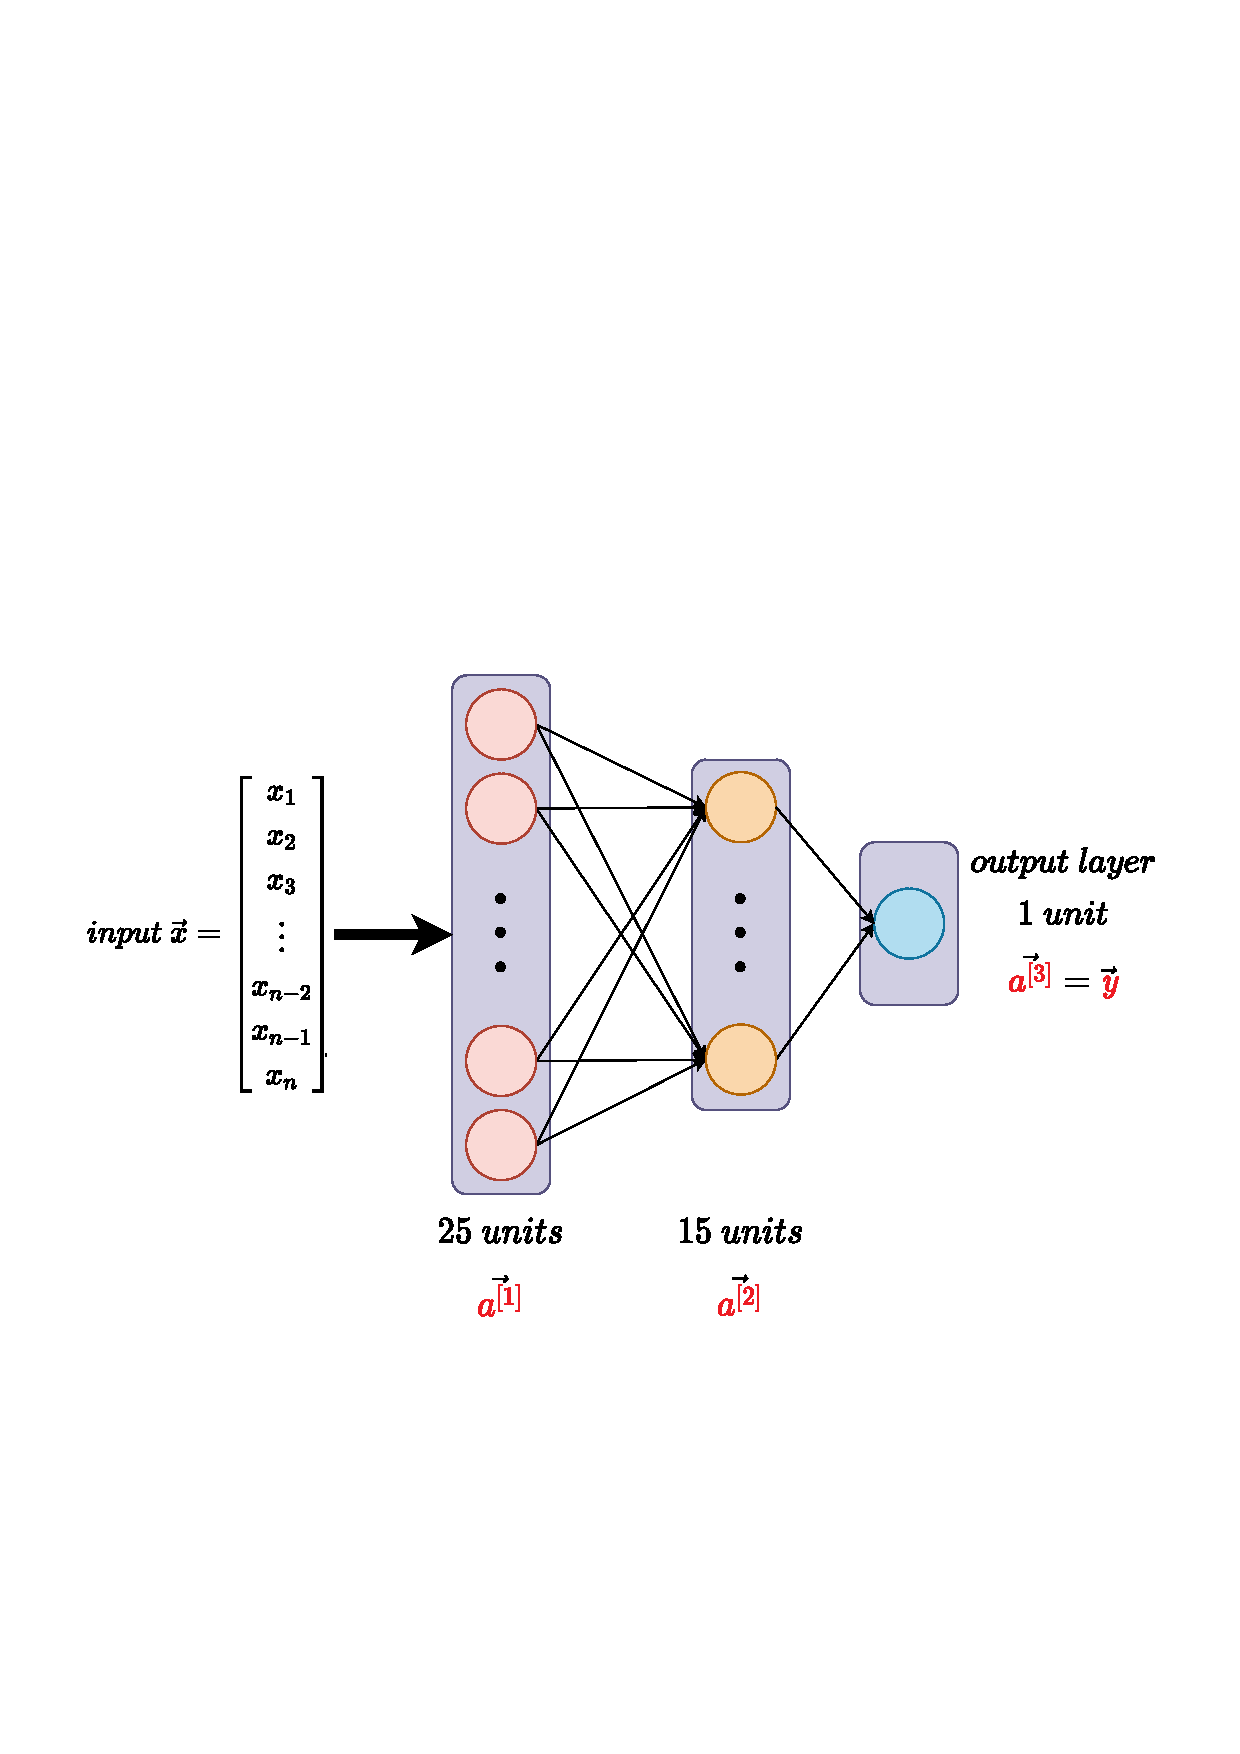
\includegraphics[width=0.4\textwidth,height=0.25\textwidth]{images/pic1.drawio.pdf}
    \caption{The Basic Architecture of a three-layer FCNN}
    \label{fig:enter-label}
\end{figure}



\begin{lstlisting}
import tensorflow as tf
from tensorflow.keras import Sequential
from tensorflow.keras.layers import Dense
model = Sequential([
        Dense(units=25,activation='sigmoid'),
        Dense(units=15,activation='sigmoid'),
        Dense(units=1,activation='sigmoid'),
    ])
from tensorflow.keras.losses import BinaryCrossentropy
model.compile(loss=BinaryCrossentropy())
model.fit(X,Y,epochs=100)
\end{lstlisting}


Several fundamental algorithms including Stochastic gradient descent(SGD)\citep{Bottou2012StochasticGD} and Back-propagation by \citet{RN32} are displayed below. 


\begin{minipage}{\linewidth}
\textbf{Algorithm I. Stochastic gradient descent(SGD)}

Inputs: loss function $\varepsilon$, learning rate $\eta$, dataset $X,y$ and the model $F(\theta,x)$.

Outputs: Optimum $\theta$ which minimizes $\varepsilon$.

REPEAT until converge:
\begin{itemize}
\item Shuffle $X,y$;
\item For each batch of $x_i,y_i$ in $X,y$ do
\begin{align*}
\tilde{y}_{i}&=\mathcal{F}\left(\theta,x_{i}\right);\\
\theta&=\theta-\eta\cdot\frac{1}{N}\sum_{i = 1}^{N}\frac{\partial\varepsilon(y_{i},\tilde{y}_{i})}{\partial\theta}
\end{align*}
\end{itemize}
\end{minipage}


\begin{minipage}{\linewidth}
\textbf{Algorithm II. Back-propagation}

Input: A network with $l$ layers, the activation function $\sigma_l$, the outputs of hidden layer $h_l=\sigma_l(W_l^T h_{l - 1}+b_l)$ and the network output $\tilde{y} = h_l$.

Compute the gradient: $\delta \leftarrow \frac{\partial \varepsilon\left(y_{i}, \tilde{y}_{i}\right)}{\partial y}$

For $i\leftarrow l$ to $0$ \textbf{do}
\begin{align*}
\frac{\partial\varepsilon(y,\tilde{y})}{\partial W_{l}}&=\frac{\partial\varepsilon(y,\tilde{y})}{\partial h_{l}}\frac{\partial h_{l}}{\partial W_{l}}=\delta\frac{\partial h_{l}}{\partial W_{l}}\\
\frac{\partial\varepsilon(y,\tilde{y})}{\partial b_{l}}&=\frac{\partial\varepsilon(y,\tilde{y})}{\partial h_{l}}\frac{\partial h_{l}}{\partial b_{l}}=\delta\frac{\partial h_{l}}{\partial b_{l}}
\end{align*}

Apply gradient descent using$\frac{\partial \varepsilon\left(y, \tilde{y}\right)}{\partial W_{l}}$and$\frac{\partial \varepsilon\left(y, \tilde{y}\right)}{\partial b_{l}}$. 
Back-propagate gradient to the lower layer
\[
\delta\leftarrow\frac{\partial\varepsilon(y,\tilde{y})}{\partial h_{l}}\frac{\partial h_{l}}{\partial h_{l - 1}}=\delta\frac{\partial h_{l}}{\partial h_{l - 1}}
\]

\end{minipage}

This article systematically reviewed the development of some classic deep neural networks of ILSVRC. The contribution lies in that we traces the development in the chronological order and summarize the general patterns of neural network development over the past decade. The survey also  conducts a statistical analysis of the number of parameters and structures of different models, which helps predicting the future development of more complex network structure.


\section{Preliminaries}


\subsection{The previous situation of Fully Connected Neural Networks(FCNNs) in Image Classification}
Before the maturation of Convolutional Neural Networks (CNNs)\citep{726791}, traditional neural networks, as the Fully Connected Neural Networks(FCNNS) faced several drawbacks and challenges.

\begin{enumerate}

\item \textbf{The Complexity of the Image Itself} 

It's difficult for machines to grab the abstract features of the images efficiently. Several images that should be classified into the same category may be diverse in colors, sizes, illumination and background clutters, which is shown in Figure 2.

Moreover, deformation and occlusion are two barriers. Deformation refers to the variations in the shape or structure of objects within images. These variations can occur due to changes in perspective, scale, or inherent flexibility of the objects themselves. Occlusion involves objects being partially obscured by other objects, which often happen in real-world scenarios.

Traditional neural networks relied on manually designed feature extraction methods, which were time-consuming and often resulted in lack of robustness to handle with the complexity of images.




\item \textbf{Severe Overfitting Problems} 

Fully Connected Neural Networks (FCNN) requires an enormous number of parameters when dealing with high-dimensional image data, leading to high computational and storage demands, making it difficult to train effectively. Due to the amount of parameters, traditional neural networks would lead to severe overfitting problems, especially when the well-labeled training data was insufficient. This meant the model performed well on the training set but poorly on the test set, leading to the model's poor generalization ability.


\begin{figure}[htb]
\centering
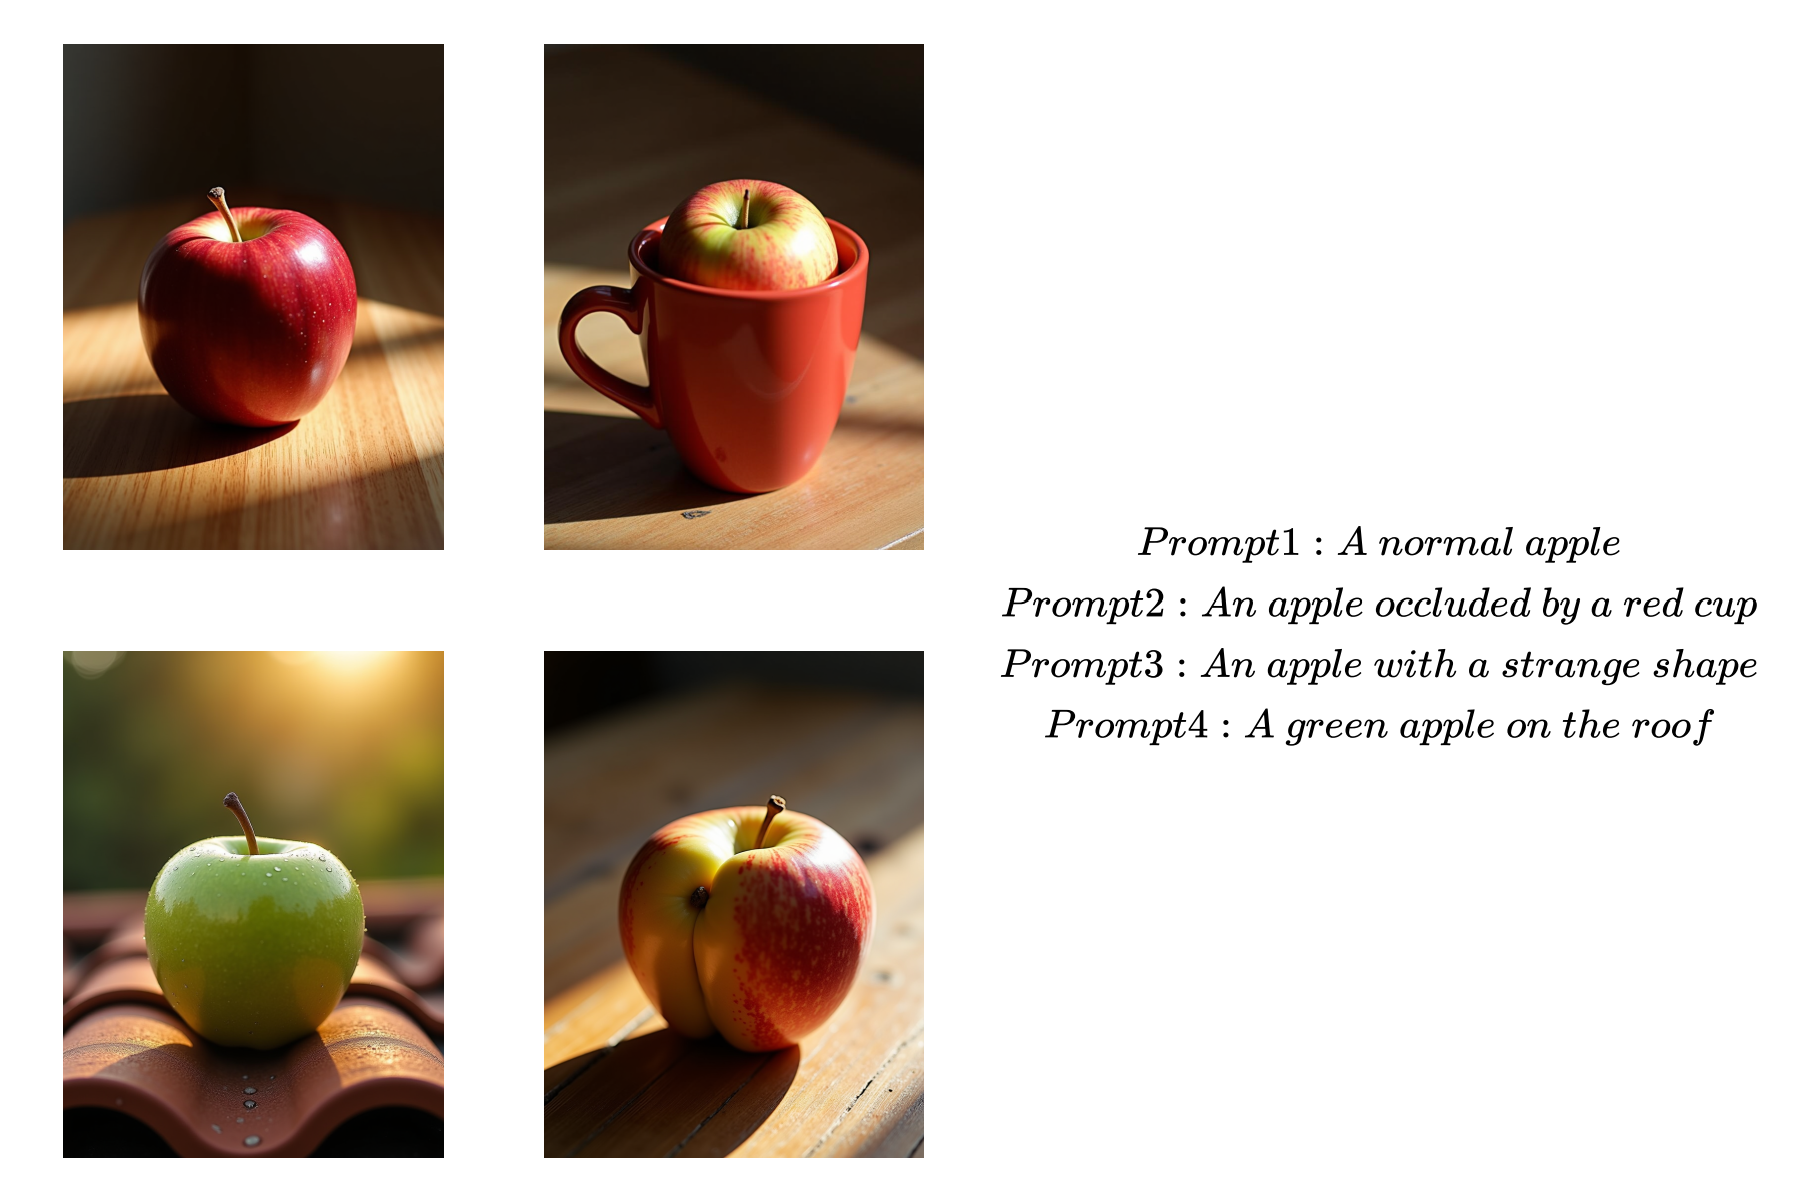
\includegraphics[width=0.4\textwidth,height=0.25\textwidth]{images/apple.png}
\hspace{0.01\textwidth}
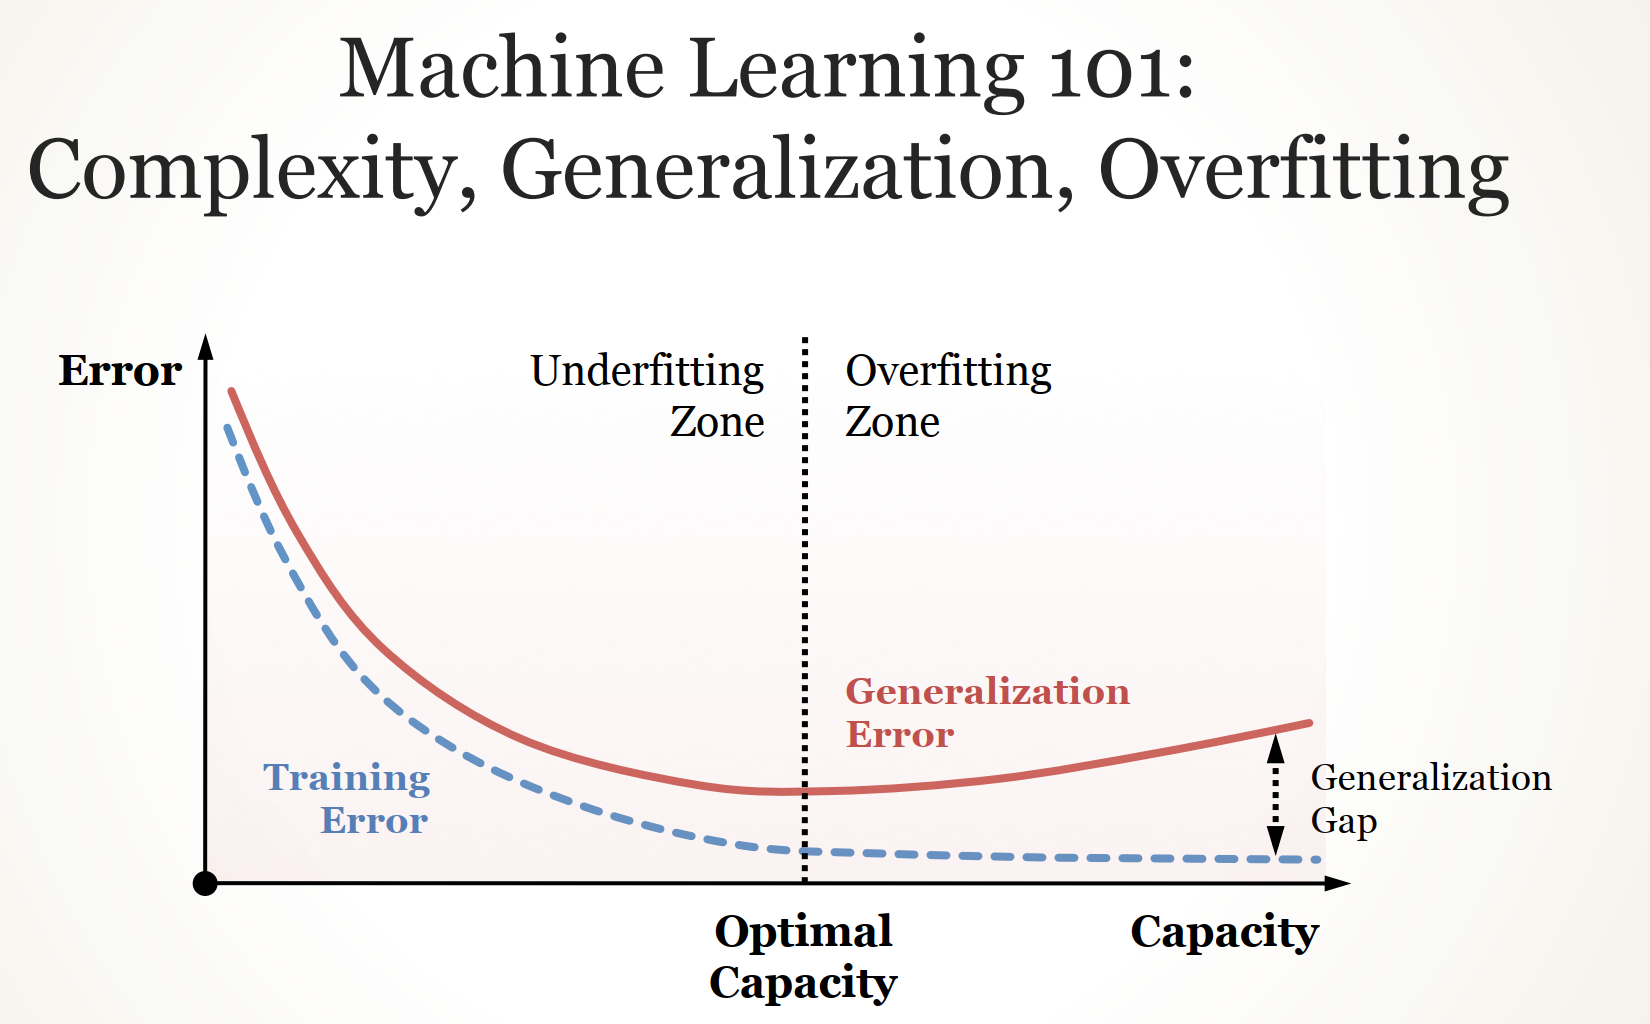
\includegraphics[width=0.4\textwidth,height=0.25\textwidth]{images/Overfitting.png}
\caption{\textbf{Left}:The complexity of the image itself, same objects with different background clutters, colours, sizes and illumination could be diverse. \textbf{Right}:Overfitting leads to the severe generalization error, where models perform badly in testset.}
%引用

\end{figure}


\end{enumerate}
\subsection{ImageNet}
The foundations of ImageNet by \citet{imagenet_cvpr09} and The ImageNet Large Scale Visual Recognition Challenge (ILSVRC) \citep{ILSVRC15} reversed the current situation and led a revival of deep neural networks. ImageNet is a large-scale visual database in visual object recognition research. It contains millions of labeled images spanning thousands of categories. Now ImageNet has 14197122 images and 21841 synsets indexed, with more detailed information in \url{https://image-net.org/}

\subsection{ImageNet Large Scale Visual Recognition Challenge(ILSVRC)}
The ImageNet Large Scale Visual Recognition Challenge (ILSVRC)\citep{ILSVRC15} has driven significant progress by providing a competitive platform for evaluating algorithms. Launched in 2010, ILSVRC provides a standardized dataset and evaluation framework for visual object recognition tasks. Participants competed to optimize the  algorithms that can accurately classify and detect objects within the vast ImageNet dataset.

The competition gained widespread attention in 2012 when AlexNet\citep{Krizhevsky2012ImageNetCW}, a deep convolutional neural network, achieved a dramatic improvement in accuracy, showcasing the potential of deep learning.ILSVRC has since become a benchmark for measuring progress in image recognition, object detection, and other related tasks.

\begin{figure}[ht]
    \centering
    % 第一个图形
    \begin{minipage}{0.4\textwidth} 
        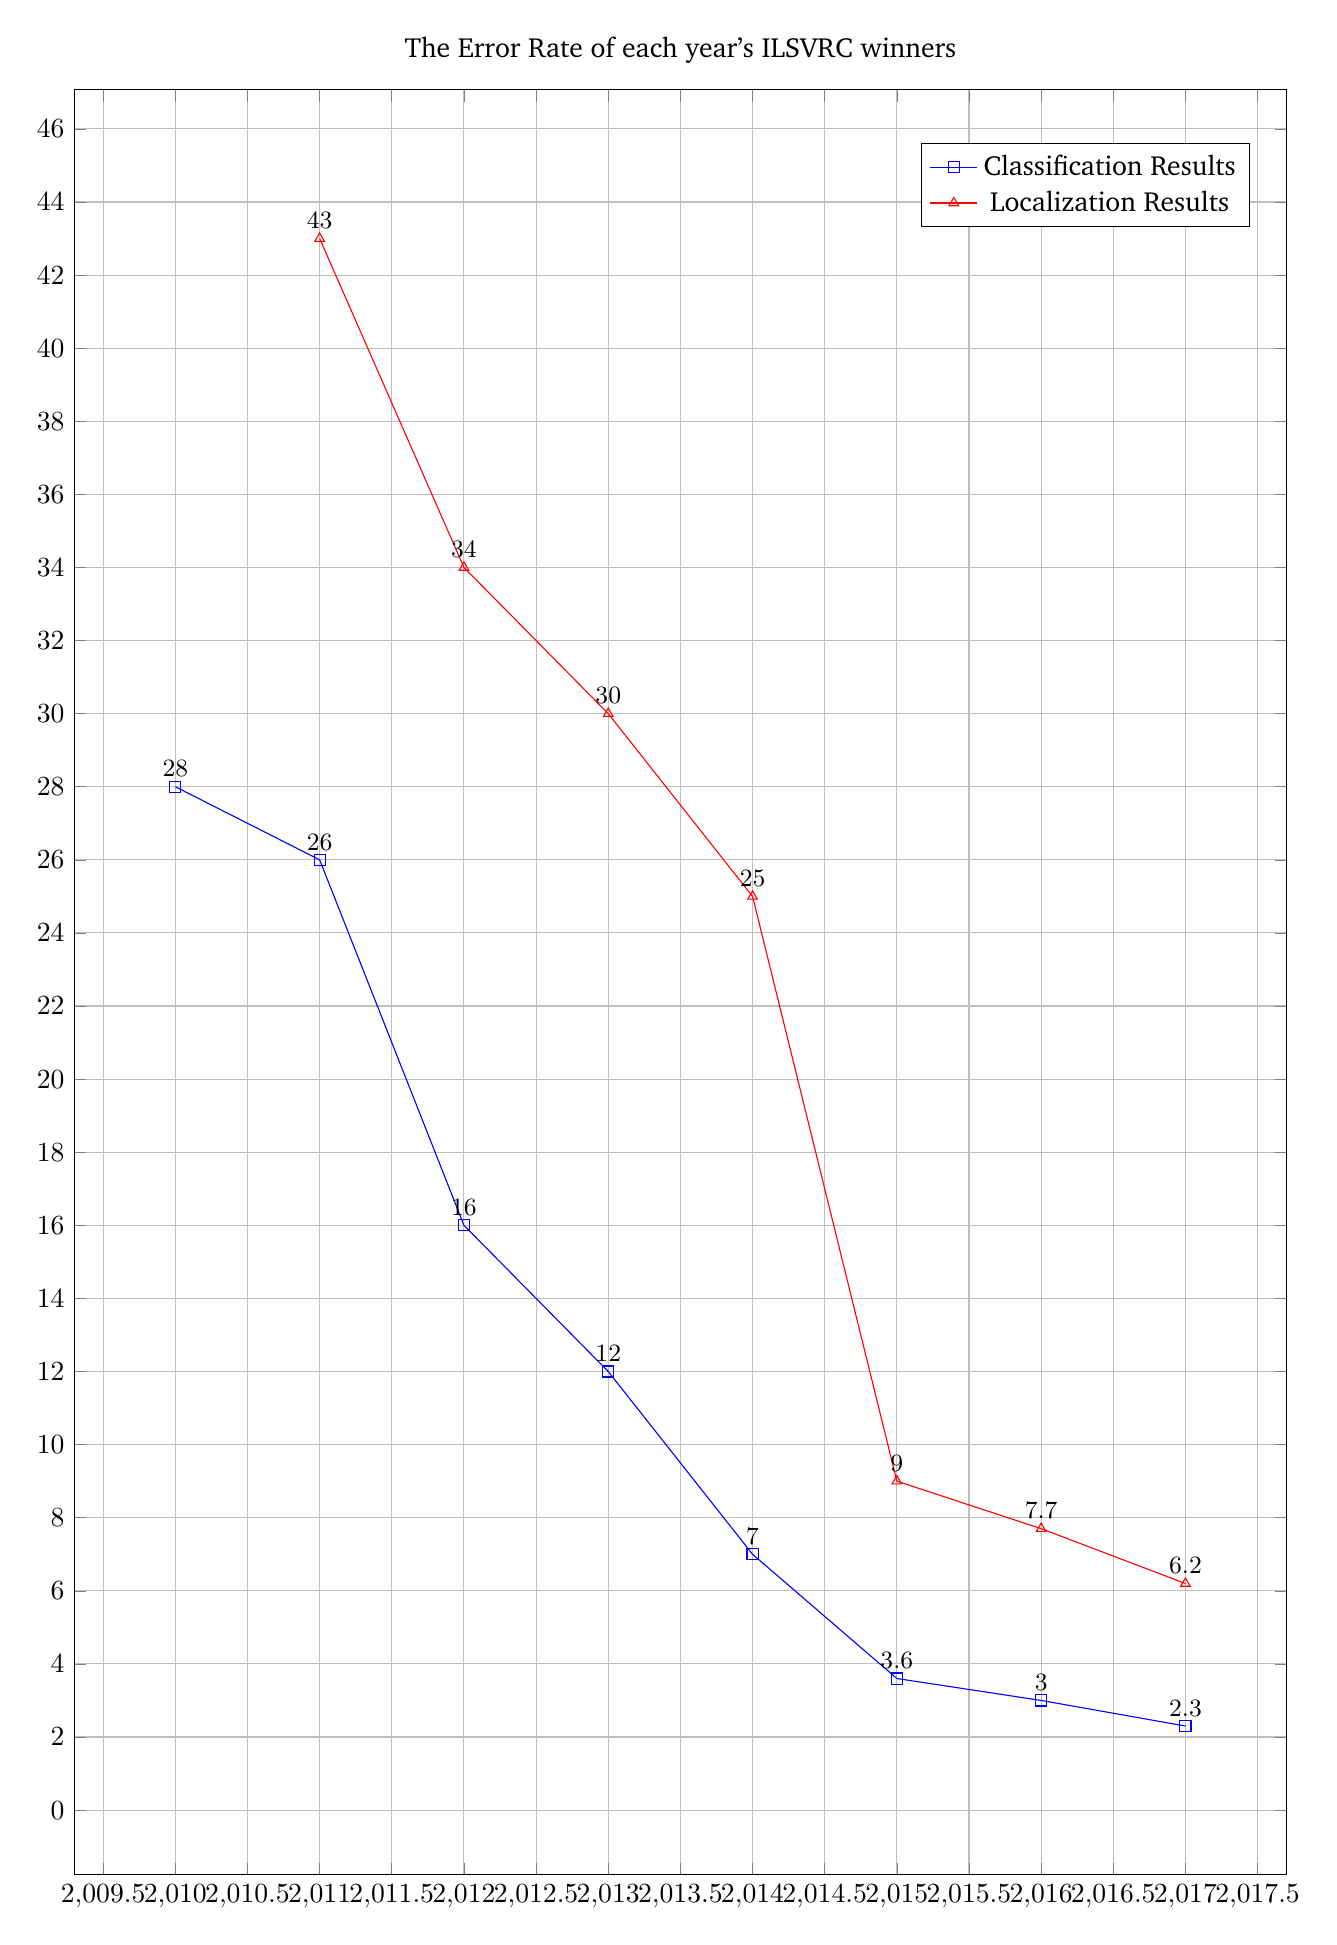
\begin{tikzpicture}
        \begin{axis}[
            title={The Error Rate of each year's ILSVRC winners},
            legend pos=north east, % 图例位置
            grid=major,
            scaled ticks=false, % 禁用科学计数法
            nodes near coords, % 显示数据标签
            every node near coord/.append style={font=\small, color=black},
            width=1.4\textwidth,
            height=2\textwidth% 标签样式    
        ]
        % 第一条折线
        \addplot[
            color=blue,
            mark=square,
            ]
            coordinates {
            (2010,28)
            (2011,26)
            (2012,16)
            (2013,12)
            (2014,7)
            (2015,3.6)
            (2016,3)
            (2017,2.3)
        };
        \addlegendentry{Classification Results} % 图例条目

        % 第二条折线
        \addplot[
            color=red,
            mark=triangle,
            ]
            coordinates {
            (2011,43)
            (2012,34)
            (2013,30)
            (2014,25)
            (2015,9)
            (2016,7.7)
            (2017,6.2)
        };
        \addlegendentry{Localization Results} % 图例条目

        \end{axis}
    \end{tikzpicture}
    \end{minipage}%
    \hspace{0.1\textwidth} % 在两个minipage之间添加空白
    % 第二个图形
    \begin{minipage}{0.35\textwidth} % 占页面宽度的45%
        \centering
    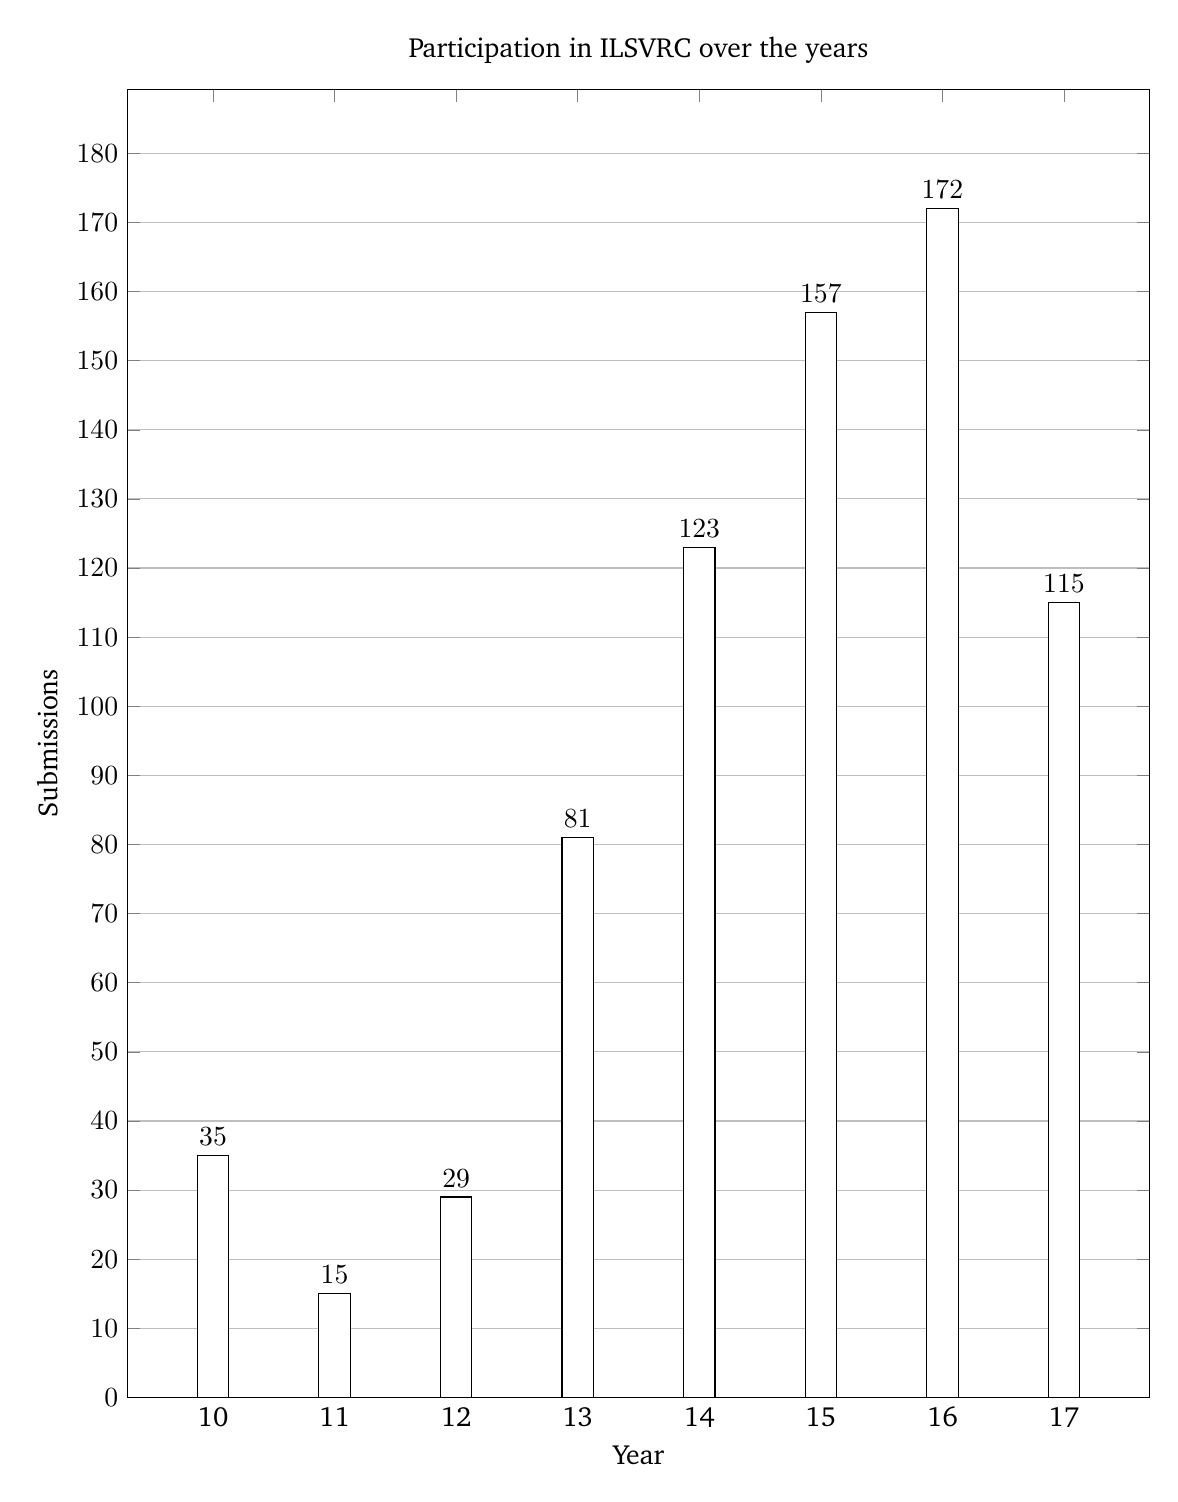
\begin{tikzpicture}
        \begin{axis}[
            title={Participation in ILSVRC over the years},
            xlabel={Year},
            ylabel={Submissions},
            ymin=0, % 设置y轴的最小值
            symbolic x coords={10, 11, 12, 13, 14,15,16,17}, % 定义分类标签
            xtick=data, % 使用数据点作为x轴刻度
            nodes near coords, % 在每个条形上显示数值标签
            bar width=0.4cm, % 设置条形的宽度
            enlarge x limits=0.10, % 增加x轴的边界
            ymajorgrids=true, % 显示y轴的网格线
            colormap name=rainbow,
            width=1.2\textwidth,
            height=1.5\textwidth
        ]
        
        \addplot[
            ybar,
            fill =white, % 设置条形的填充颜色
            ]
            coordinates {
                (10, 35)
                (11, 15)
                (12, 29)
                (13, 81)
                (14, 123)
                (15,157)
                (16,172)
                (17,115)
            };

        \end{axis}
    \end{tikzpicture}
    \end{minipage}
    \caption{The error rate and the submissions of each year's ILSVRC challenges, from \url{https://image-net.org/challenges/beyond_ilsvrc.php}}
\end{figure}


%添加表格

\subsection{Convolutional Neural Networks(CNNs) and LeNet}
Convolutional Neural Network (CNN) is a type of deep learning model specifically designed for processing structured data, such as images. CNNs are particularly effective for image recognition and classification tasks due to their ability to learn spatial hierarchies of features. 

Convolutional neural networks were originally proposed by \citet{726791}, specialized for handwriting characters recognition. The architecture of a CNN typically includes multiple layers, including convolutional layers, pooling layers, and fully connected layers.

\begin{enumerate}
\item \textbf{Convolutional Layers} These layers apply convolution operations to the input, using filters (kernels) to create feature maps that capture spatial hierarchies. In a convolutional layer, the primary operation is the convolution, where a small matrix of weights, known as a filter or kernel, slides over the input image. This operation computes dot products between the filter and local patches of the input, producing feature maps. Filters are learned during training and detect specific features such as edges, textures, and patterns. Multiple filters can be applied to capture various features.
\item \textbf{Pooling Layers} Pooling layers perform down-sampling operations, reducing the dimension of the feature maps and making the network more computationally efficient while retaining important information. The most common type is Max Pooling\citep{726791}, which selects the maximum value in each patch of the feature map, and Average Pooling and Global Average Pooling\citep{Lin2013NetworkIN}, which computes the average value.
\item \textbf{Fully Connected Layers} These layers are similar to traditional neural networks and connect every neuron in one layer to every neuron in the next layer. After catching the different features of the image by using previous Convolutional and Pooling layers, the fully connected layers integrated several features into a single value, ignoring the influence that the position of the image brings, thus significantly enhanced the robustness of the model.
\end{enumerate}

\begin{figure}[ht]
    \centering
    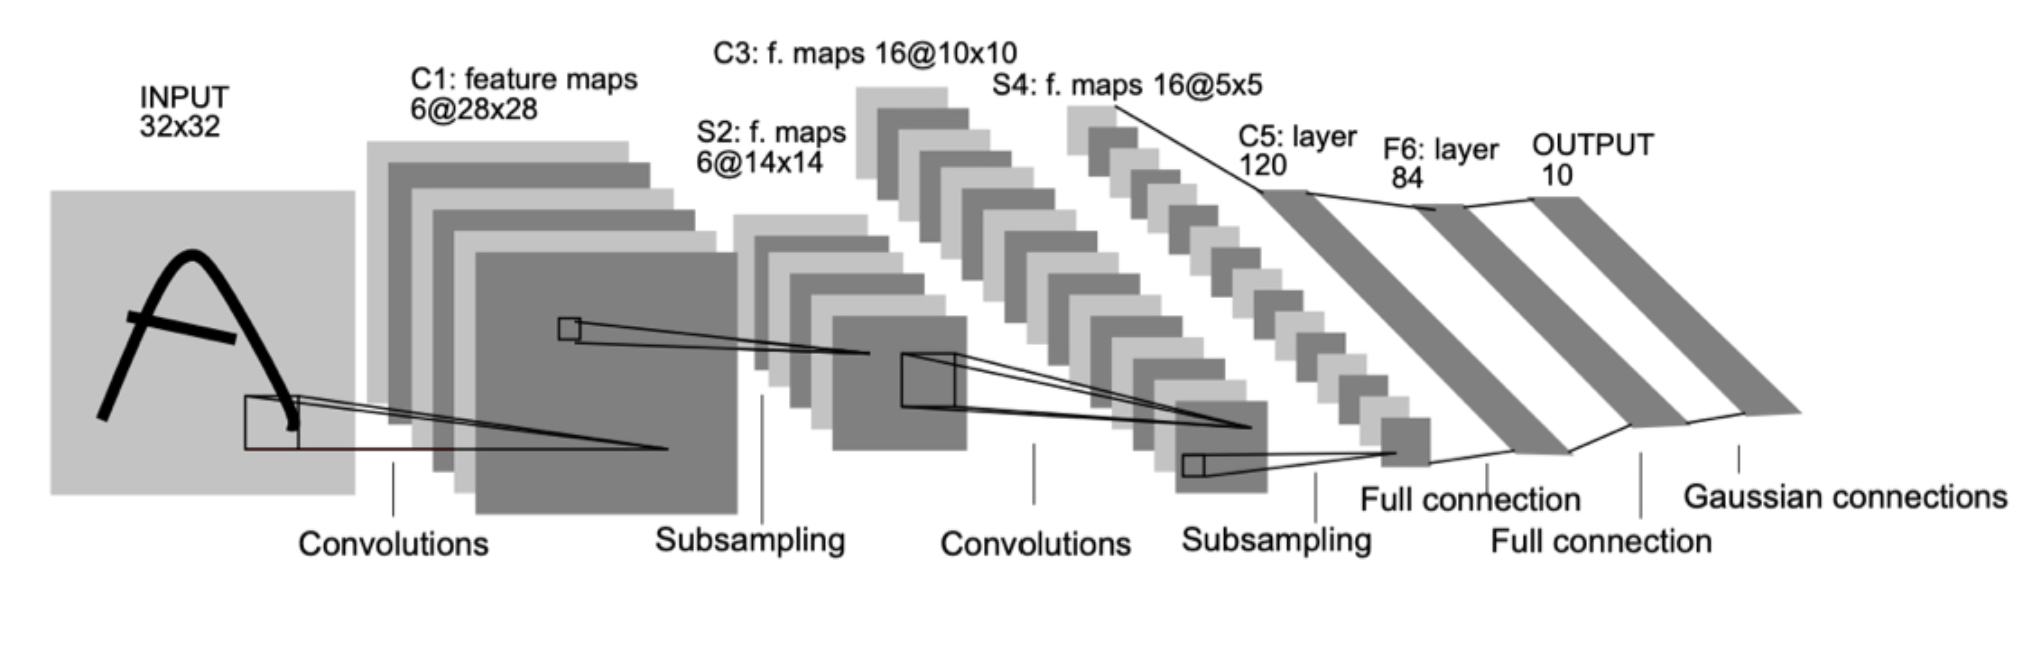
\includegraphics[width=0.7\textwidth,height=0.25\textwidth]{images/Lenet.png}
    \caption{The structure of LeNet\citet{726791}}
\end{figure}


\section{A Decade of Breakthroughs: Key Winners of the ILSVRC Competition}

Launched in 2010,The ImageNet Large Scale Visual Recognition Challenge(ILSVRC) has generated countless outstanding achievements, including \textbf{AlexNet(2012)}\citep{Krizhevsky2012ImageNetCW}, \textbf{ZFNet(2013)}\citep{DBLP:journals/corr/ZeilerF13}, \textbf{GoogLeNet(2014)}\citep{DBLP:journals/corr/SzegedyLJSRAEVR14}, \textbf{ResNet(2015)}\citep{DBLP:journals/corr/HeZRS15} and \textbf{ResNeXt(2016)}\citep{DBLP:journals/corr/XieGDTH16}


\subsection{2012: AlexNet – The Breakthrough of Deep Learning}

AlexNet's architecture was quite similar to LeNet, but with the efficient use of multiple GPUs, the well-structured data and the enormous amount of labeled data of ImageNet, AlexNet significantly decreased the error rate to 15.3\%. Consisting five convolutional layers, three fully-connected layers and a final 1000-way softmax output layers, AlexNet used stochastic gradient descent (SGD)\citep{DBLP:journals/corr/Ruder16} with a batch size of 128 examples, momentum of 0.9, and weight decay of 0.0005. The following graph shows a illustration of the architecture of AlexNet.

\begin{figure}[ht]
    \centering
    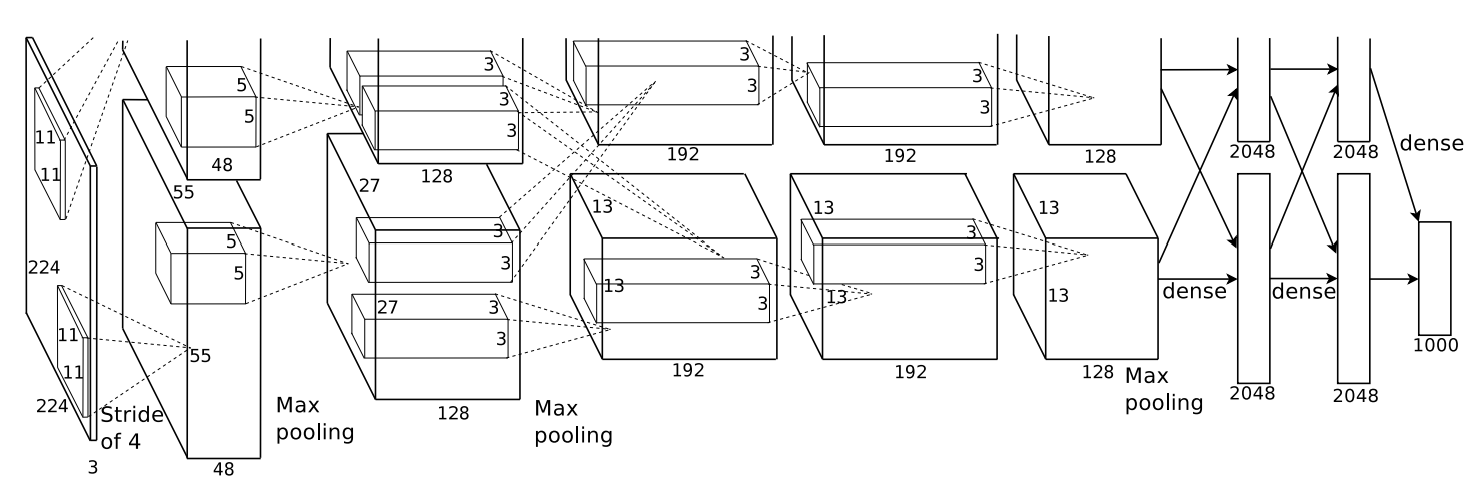
\includegraphics[width=0.7\textwidth,height=0.25\textwidth]{images/Alexnet.png}
    \caption{The Structure of AlexNet\citep{Krizhevsky2012ImageNetCW}}
\end{figure}

AlexNet also used quite a few optimization methods so as to minimize the error rate of the CNN, including the ReLU activation, the Local Response Normalization(LRN) and the innovative use of Dropout.


\begin{enumerate}
    \item \textbf{The ReLU activation}
    The previous activation function used by previous convolutional was mainly the saturating nonlinearities including $f(x)=\tanh x$ and sigmoid function $f(x)=\frac{1}{1+e^{-x}}$. However, these saturating nonlinearities have much more complex computational process, while using the Rectified Linear Units (ReLUs)\citep{Nair2010RectifiedLU} $f(x)=\max \{0,x\}$ has much more advantages. With the ReLU activation, the training process requires less computational process, and effectively solves the problem of gradient descent and gradient vanishing on certain intervals.
    \item \textbf{the Local Response Normalization(LRN)}
    Local Response Normalization was an efficient method for enhancing the accuracy when training the convolutional neural networks, imitating the lateral inhibition in neurons. The specific expression was as below.
    $$b_{x, y}^{i}=a_{x, y}^{i} /\left(k+\alpha \sum_{j=\max (0, i-n / 2)}^{\min (N-1, i+n / 2)}\left(a_{x, y}^{j}\right)^{2}\right)^{\beta}$$
    LRN makes the correlation between feature maps generated by different convolutional kernels smaller by introducing competition between feature maps generated by neighboring convolutional kernels.
    \item \textbf{Dropout}
    Dropout is a technique dropping the output of each hidden neuron to zero with probability of 0.5. So every time an input is presented, the neural network samples a different architecture, but all these architectures share weights, allowing the network to learn more robust features and effectively solves the overfitting problem.
\end{enumerate}

\subsection{2014: GoogLeNet – The Power of Inception}
GoogLeNet\citep{DBLP:journals/corr/SzegedyLJSRAEVR14}\citep{DBLP:journals/corr/SzegedyVISW15}, the winner of ILSVRC2014, proposed a deep convolutional neural network architecture named Inception and increased the depth and width of the networks while keeping the computational budget constant. This net effectively clusters sparse matrices into denser submatrices to improve computational performance, managing to decrease the error rate(Top-5) to 6.67\%.More detailed information of the algorithm can be seen in \url{https://github.com/conan7882/GoogLeNet-Inception}


\begin{table}[ht]
\caption{The Basic architecture of GoogLeNet}
\resizebox{\textwidth}{!}{
\begin{tabular}{c|ccc|c|c|c|c|c|c|cc}
\hline
\textbf{type}  & \textbf{patch size/ stride} & \textbf{output size} & \textbf{depth} & \#1×1                 & \#3×3reduce           & \#3×3 & \#5×5reduce           & \#5×5                 & \textbf{pool proj} & \textbf{params} & \textbf{ops} \\ \hline
convolution    & 7×7/2                       & 112×112×64           & 1              & \multicolumn{1}{l|}{} & \multicolumn{1}{l|}{} &       &                       &                       &                    & 2.7K            & 34M          \\ \hline
max pool       & 3×3/2                       & 56×56×64             & 0              &                       &                       &       &                       &                       &                    &                 &              \\ \hline
convolution    & 3×3/1                       & 56×56×192            & 2              & \multicolumn{1}{l|}{} & 64                    & 192   & \multicolumn{1}{l|}{} & \multicolumn{1}{l|}{} &                    & 112K            & 360M         \\ \hline
max pool       & 3×3/2                       & 28×28×192            & 0              &                       &                       &       &                       &                       &                    &                 &              \\ \hline
inception (3a) &                             & 28×28×256            & 2              & 64                    & 96                    & 128   & 16                    & 32                    & 32                 & 159K            & 128M         \\ \hline
inception (3b) &                             & 28×28×480            & 2              & 128                   & 128                   & 192   & 32                    & 96                    & 64                 & 380K            & 304M         \\ \hline
max pool       & 3×3/2                       & 14×14×480            & 0              &                       &                       &       &                       &                       &                    &                 &              \\ \hline
inception (4a) &                             & 14×14×512            & 2              & 192                   & 96                    & 208   & 16                    & 48                    & 64                 & 364K            & 73M          \\ \hline
inception (4b) &                             & 14×14×512            & 2              & 160                   & 112                   & 224   & 24                    & 64                    & 64                 & 437K            & 88M          \\ \hline
inception (4c) &                             & 14×14×512            & 2              & 128                   & 128                   & 256   & 24                    & 64                    & 64                 & 463K            & 100M         \\ \hline
inception (4d) &                             & 14×14×528            & 2              & 112                   & 144                   & 288   & 32                    & 64                    & 64                 & 580K            & 119M         \\ \hline
inception (4e) &                             & 14×14×832            & 2              & 256                   & 160                   & 320   & 32                    & 128                   & 128                & 840K            & 170M         \\ \hline
max pool       & 3×3/2                       & 7×7×832              & 0              &                       &                       &       &                       &                       &                    &                 &              \\ \hline
inception (5a) &                             & 7×7×832              & 2              & 256                   & 160                   & 320   & 32                    & 128                   & 128                & 1072K           & 54M          \\ \hline
inception (5b) &                             & 7×7×1024             & 2              & 384                   & 192                   & 384   & 48                    & 128                   & 128                & 1388K           & 71M          \\ \hline
avg pool       & 7×7/1                       & 1×1×1024             & 0              &                       &                       &       &                       &                       &                    &                 &              \\ \hline
dropout (40\%) &                             & 1×1×1024             & 0              &                       &                       &       &                       &                       &                    &                 &              \\ \hline
linear         &                             & 1×1×1000             & 1              & \multicolumn{1}{l|}{} & \multicolumn{1}{l|}{} &       &                       &                       &                    & 1000K           & 1M           \\ \hline
softmax        &                             & 1×1×1000             & 0              &                       &                       &       &                       &                       &                    &                 &              \\ \hline
\end{tabular}

}

    \label{tab:your_label}
\end{table}
\begin{figure}[ht]
    \centering
    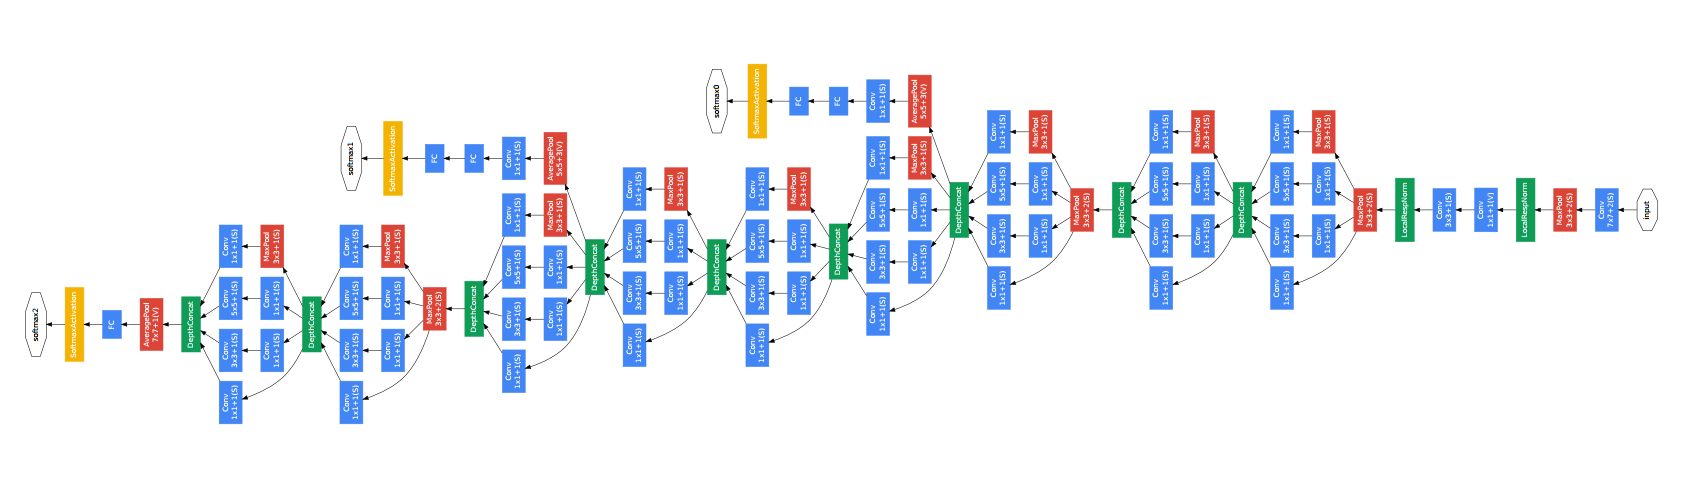
\includegraphics[width=\textwidth]{images/GooGLenet.png}
    \caption{The Structure of GoogLeNet\citep{DBLP:journals/corr/SzegedyLJSRAEVR14}}
\end{figure}


Several innovations of GoogLenet are as follows.
\begin{enumerate}
    \item \textbf{The Inception Models}
    In traditional Convolutional Neural Networks like Alexnet and VGGNet, a series of convolutional and pooling layers are connected sequentially, leading to the huge amount of the parameters. Inception applies multiple types of convolutional filters (such as 1$\times$1, 3$\times$3, and 5$\times$5) within the same layer. As clustering sparse matrices into denser matrices can improve computational performance, different convolutional operations are performed in parallel, where the input data is processed simultaneously by different filters, and the results are concatenated along the depth dimension to form a unified output. Moreover, adapting more 1$\times$1 convolutional filters can decrease the dimension of the model, making the network compute less parameters especially when using a 5$\times$5 convolutional kernels.

    Using the Inception module can increase network depth without excessive parameters and reduce the computational process, thus overcoming the severe overfitting problems.
    
    
    \item \textbf{Global Average Pooling}
    Despite the inception-v1 modules, GoogLeNet also replaced the fully connected layers into global average pooling layers, which averages the feature maps across their spatial dimensions. Fully Connected Layers are responsible for classifying the features extracted from the convolutional layer with activation function such as softmax, which are often equipped with enormous parameters. But the GAP with no need of parameter performs average pooling for each feature map by averaging all the pixel values of the entire feature map and feeds the resulting vector directly into the softmax layer to output the classification.


    \begin{figure}[ht]
    \centering
    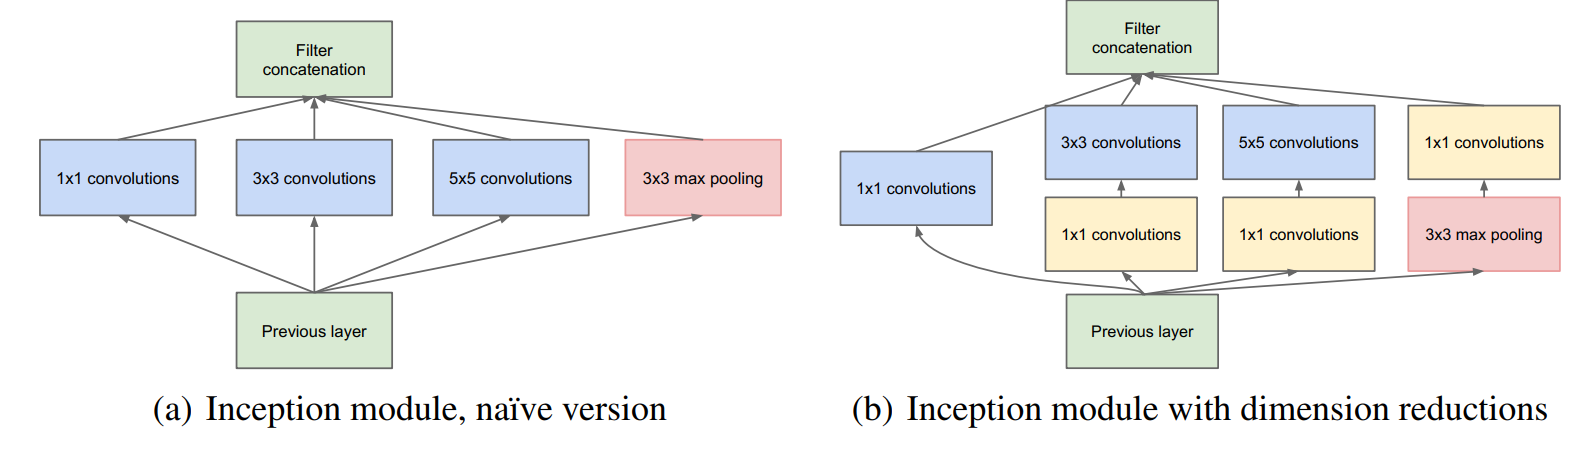
\includegraphics[width=0.8\textwidth,height=0.25\textwidth]{images/Inception.png}
    \caption{The Inception Module, where different dimensions of convolutional kernels and pooling layers are added.\citep{DBLP:journals/corr/SzegedyLJSRAEVR14}}
\end{figure}

\begin{table}[ht]
\caption{The depth and the parameters of LeNet, AlexNet and GoogLeNet}
\begin{tabular}{l|lllll}
\hline
\multicolumn{1}{c|}{Model} & Depth & Convolutional Layers & Fully Connected Layers & Parameters & Error Rate \\ \hline
LeNet     & 7  & 3  & 1 & 0.06M &        \\ \hline
AlexNet   & 8  & 5  & 3 & 60M   & 15.3\% \\ \hline
GoogLeNet & 22 & 10 &   & 5M    & 6.67\% \\ \hline
\end{tabular}

\end{table}

\end{enumerate}

\subsection{2015-2016: ResNet and ResNeXt – Tackling the Depth of Networks}
The rapid development of Inception enables deep neural networks to have much deeper layers with relatively fewer parameters. However, \citet{DBLP:journals/corr/HeZRS15} found the degradation phenomenon, as deeper networks preform poorly in comparison with networks with shallow layers. Unexpectedly, such degradation is not caused by overfitting, and adding more layers to a suitably deep model leads to higher training error as is shown in the graph below.

 
\begin{figure}[ht]
    \centering
    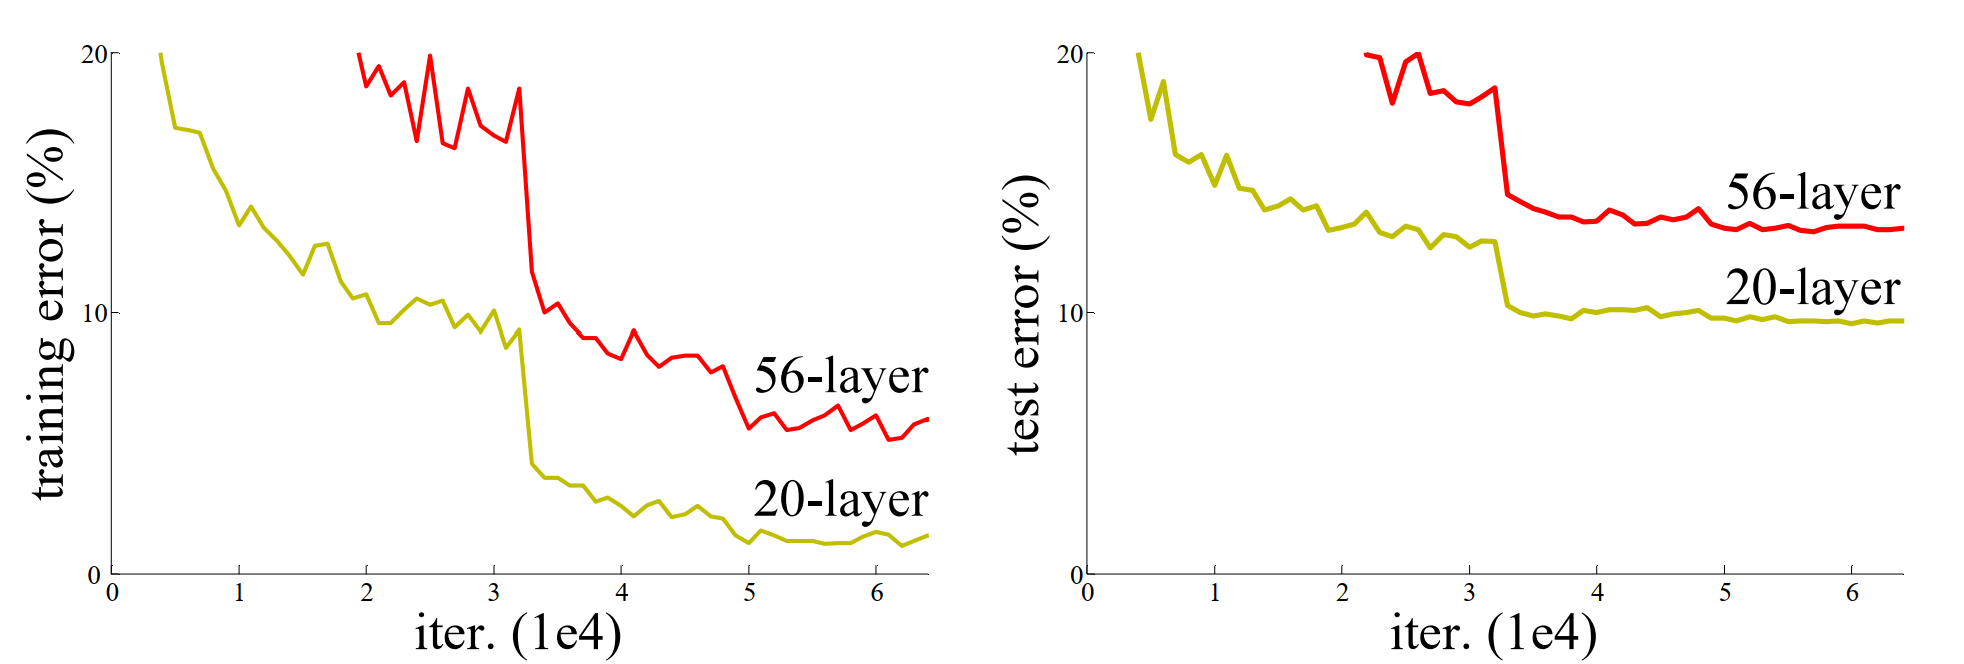
\includegraphics[width=0.7\textwidth,height=0.25\textwidth]{images/ResNet1.png}
    \caption{Training error (left) and test error (right) on CIFAR-10
with 20-layer and 56-layer “plain” networks. The deeper network
has higher training error, and thus test error. \citep{DBLP:journals/corr/HeZRS15}}

\end{figure}

The research team addressed the degradation problem by introducing a deep residual neural network. With the aim of letting a deeper model produce no higher training error than its shallower counterpart, the deep residual neural network added several identity mapping layers $g(x):=x$, known as the shortcut connections, letting the stacked nonlinear layers fit the residual mapping of $f(x):=\mathcal{F} (x)-x$. Thus the original mapping $\mathcal{F} (x)$ is the sum of the residual mapping and the added identity mapping, enabling less training error when increasing the depth of CNNs without introducing neither extra parameters nor computation complexity.

For every building block in deep residual neural network, the output vectors can be computed as below.$$\mathbf{y}=\mathcal{F}\left(\mathbf{x},\left\{W_{i}\right\}\right)+W_{s} \mathbf{x}$$

The linear projection matrix $W_{s}$ is used for adapting the input vector into different dimensions. As for the overall architecture of ResNet, ResNet is equipped with 50(ResNet-50), 101(ResNet-101), 152(ResNet-152) or much more layers with a lower error rate of 3.57\% in ILSVRC2015. More details regarding the code can be seen in \url{https://github.com/facebookarchive/fb.resnet.torch?tab=readme-ov-file}

\begin{figure}[ht]
    \centering
    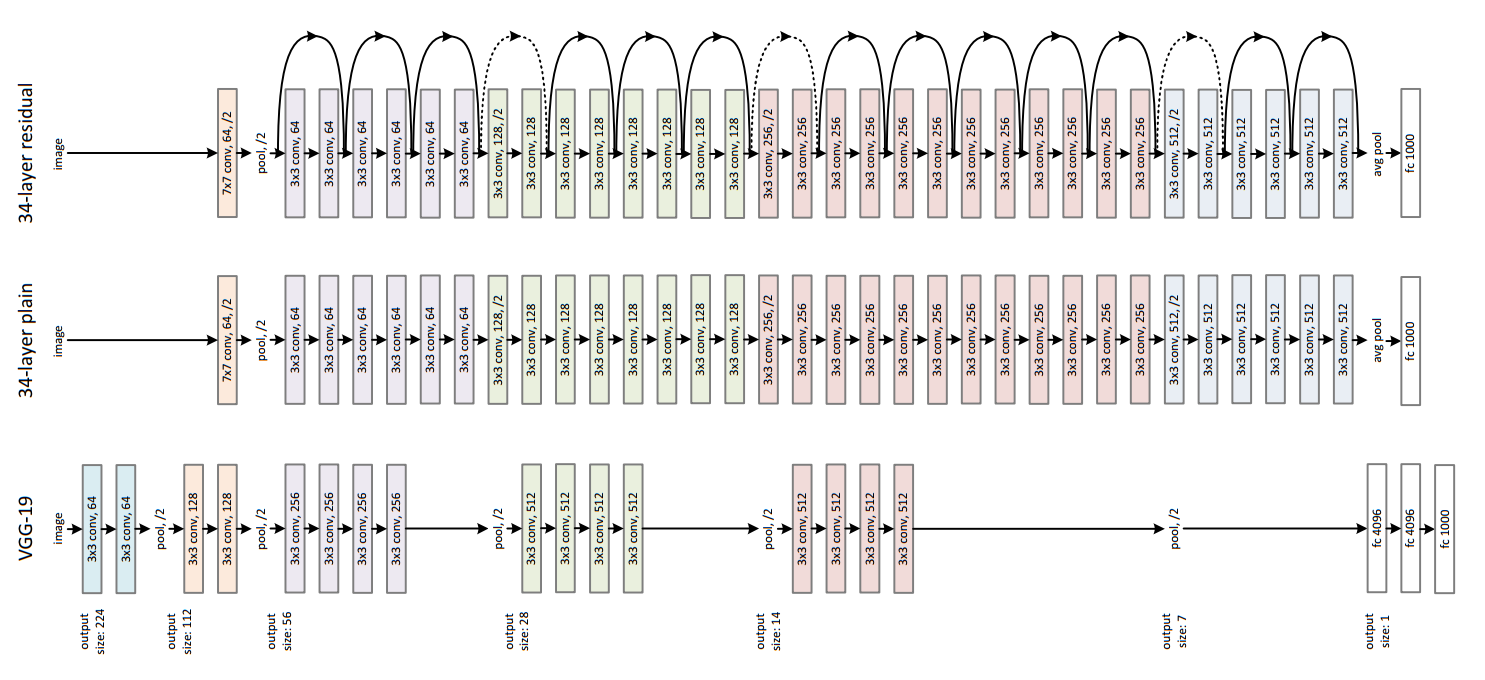
\includegraphics[width=\textwidth]{images/ResNet2.png}
    \caption{The Architecture of Deep Residual Neural Network\citep{DBLP:journals/corr/HeZRS15}}
\end{figure}

\begin{figure}[ht]
    \centering
    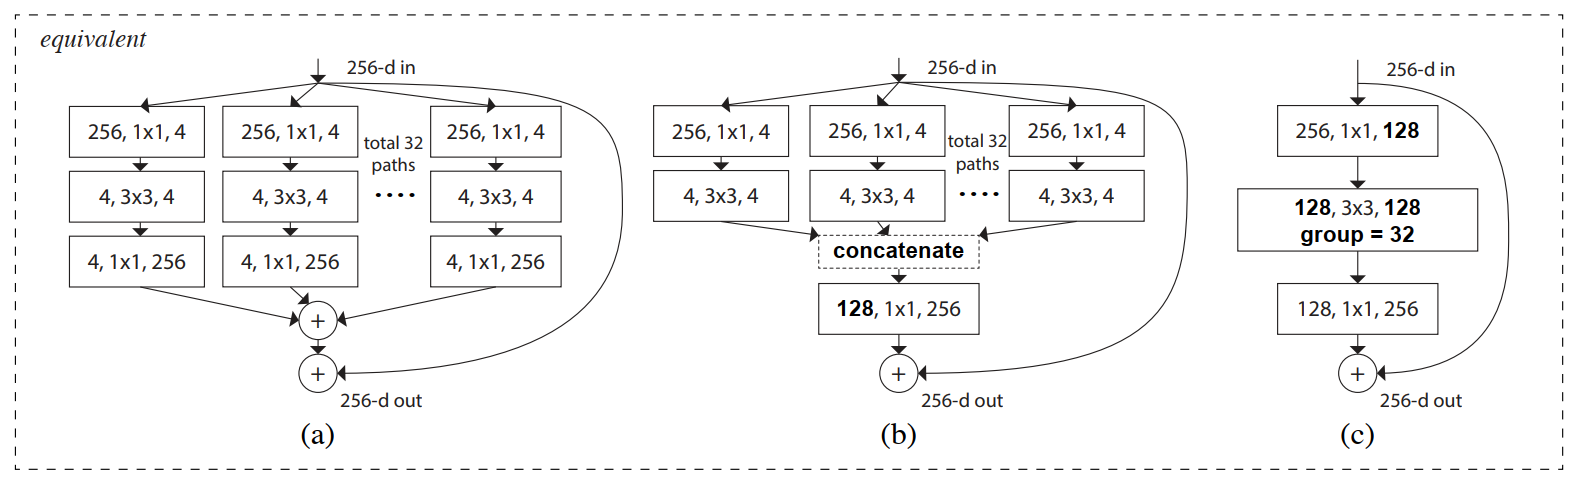
\includegraphics[width=\textwidth]{images/ResNeXt.png}
    \caption{The Architecture of ResNeXt\citep{DBLP:journals/corr/XieGDTH16}}
\end{figure}

In ILSVRC2016, the research team launched ResNeXt as an improved version of ResNet. ResNeXt is built upon the ResNet architecture by introducing a new dimension called "cardinality", which refers to the number of parallel paths within a residual block. Unlike ResNet, which focuses on increasing the depth (number of layers) and width (number of channels), ResNeXt increases the cardinality to enhance model capacity and performance. Each block in ResNeXt consists of multiple parallel convolutional paths, each with a smaller number of filters, and their outputs are aggregated by $\mathbf{y}=\mathbf{x}+\sum_{i=1}^{C} \mathcal{T}_{i}(\mathbf{x})$. By leveraging grouped convolutions, ResNeXt efficiently reduced the error rate to 3\% while maintaining the simplicity of the original ResNet design. 




\section{The Impact and Outlook}

\subsection{Tracing the Development of Deep Neural Network}

The development of deep convolutional neural networks was significant during the last decade. The graph shows the pros and cons of several classic networks in ILSVRC challenges.

\begin{figure}[ht]
    \centering
    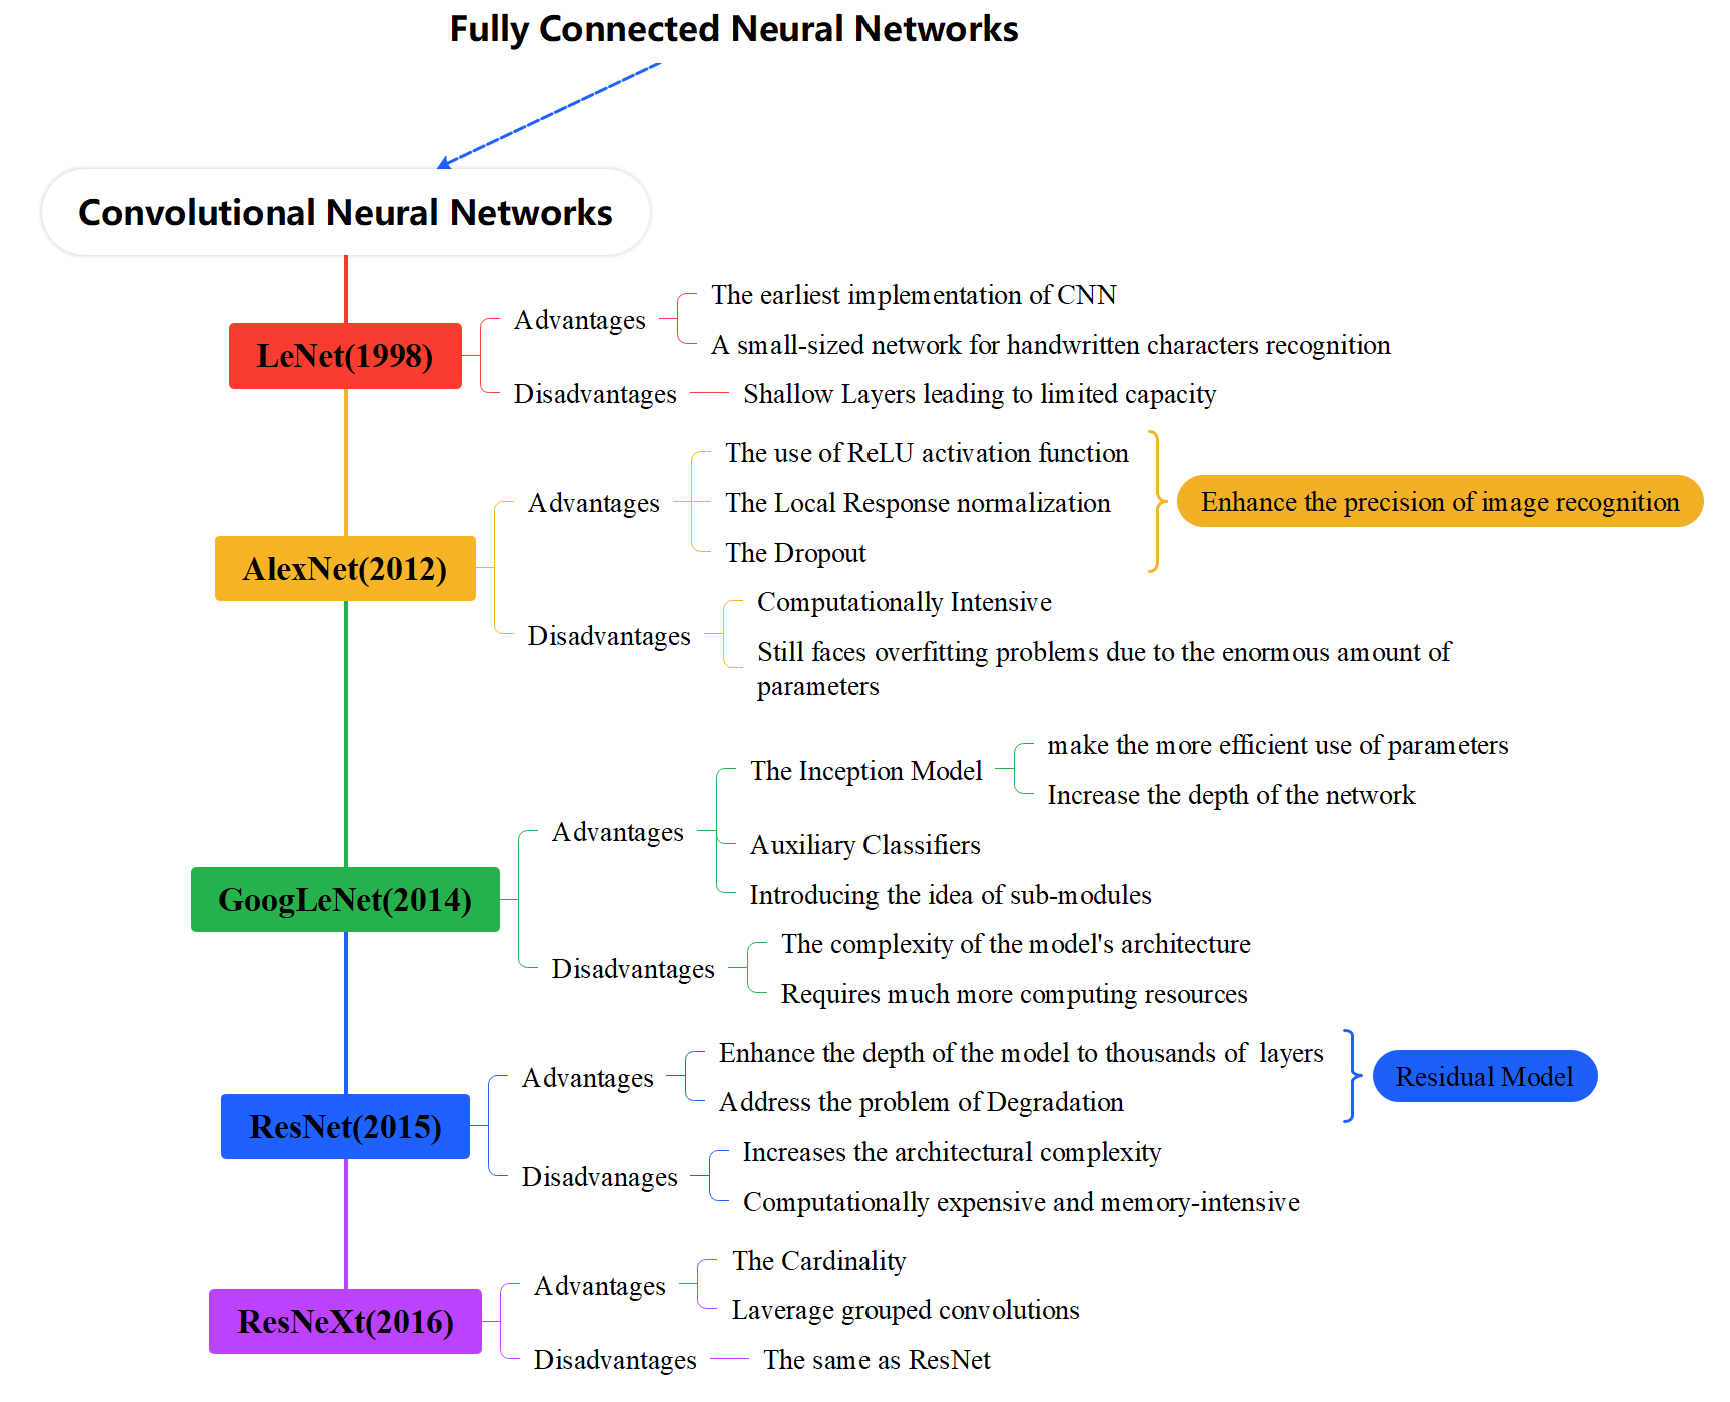
\includegraphics[width=\textwidth]{images/siwei.png}
    \caption{The pros and cons of several classic neural networks in ILSVRC}
\end{figure}

Tracing the development of ILSVRC winners each year, the ultimate goal for all deep neural networks is to find a innovative architecture to outperform the result of image classification, as enhancing the network's capacity while reducing computational complexity and address several problems like overfitting.

As for the issue to enhance the model's capacity, the convolutional neural network is the basic structure, enabling to get the abstract features of images and addressing the problem of the variations in the shape or structure of objects within images. And several networks such as AlexNet increase the amount of parameters and the depth of networks, thus enhancing the performance in image classification.

But simply expanding the size of the networks would lead to complexity both structurally and computationally, as well as the overfitting problem. So an important direction for optimization is how to reduce the number of parameters and decrease the generization error, including the ReLU activation, Dropout and Global Average Pooling. Several models after GoogLeNet also innovated several sub-modules such as the Inception, the Residual model and the cardinality, which could advance the performance without introducing new parameters. This addresses problems such as degradation and overfitting, which often appears in large-sized CNNs.

However, as of now, these convolutional neural networks suffer from problems such as overly complex model structures, poor visualization, and the need for large amounts of computational resources such as GPUs. In the future, we have the potential to design neural networks that are lighter but achieve the same performance.

\subsection{For Future Outlook}

The winners of \href{https://image-net.org/challenges/LSVRC/2017/index.php}{ILSVRC2017} have decreased the error rate into 2.3\%(top-5), which is much lower than human's behaviour. So which direction we should take to embrace the next decade Neural Network Innovation?

\begin{enumerate}
    \item \textbf{Striving for Higher Quality Datasets}
    After ImageNet, several datasets such as \href{https://cocodataset.org/}{COCO(Common Objects in Context)} and \href{https://storage.googleapis.com/openimages/web/index.html}{Open Image Datasets} by GoogLe have emerged to push the boundaries further in image classification. The high quality of well-labeled data could enhance the robustness of the model. 
    \item \textbf{The move from object recognition to human-level understanding}
    Deep Neural Networks could be applied in many extensive fields, far more than simply classifying images into several categories. For example a dataset called Visual Genome \citep{DBLP:journals/corr/KrishnaZGJHKCKL16} focuses on understanding images in a more detailed manner, providing annotations for objects, attributes, and relationships between objects within images.
    \item \textbf{The fundamental innovation of Convolutional Neural Network}
    Nearly all the winners' models of ILSVRC were based on the fundamental CNN structure. Could we find an alternative underlying model that outperforms convolutional neural networks? Nowadays, new architectures such as Vision Transformers(ViTs) \citep{DBLP:journals/corr/abs-2010-11929}, Momentum Contrast(MoCo)\citep{DBLP:journals/corr/abs-1911-05722}, Simple Contrastive Learning(SimCLR)\citep{DBLP:journals/corr/abs-2002-05709} and Contrastive Language-Image Pre-Training(CLIP)\citep{chen2024contrastivelocalizedlanguageimagepretraining}. These models have the advantages over traditional convolutional neural networks,such as the ability to train unlabeled data.
\end{enumerate}


\section{Conclusion}

This paper presents an overview of the development of deep neural networks over the past decade, especially the optimization of convolutional neural network. We lay emphasis on several classical CNN architectures which are the winners of ILSVRC challenges, including AlexNet, GoogLeNet, ResNet and ResNeXt. Tracing the development of these models, we then summarize the basic guiding principle of the optimization by adding the depth of the layers without introducing a huge amount of extra parameters and computational complexity.In the next decade, several feasible directions for Neural Network have proven to be successful, including striving for higher quality datasets, moving from object recognition to human-level understanding and finding alternative models outperforming traditonal CNNs.

\newpage
\bibliographystyle{apalike}
\bibliography{Paper_summaries}
\end{document}

